\documentclass[UTF8,11pt]{ctexart}
\usepackage[a4paper,margin=22mm]{geometry}
\usepackage{graphicx,enumitem,amssymb,tabularx}
\usepackage[normalem]{ulem}
\usepackage{xeCJKfntef}
\setlength{\parindent}{0pt}
\setlength{\parskip}{.6em}
\sloppy
\begin{document}
\section*{2020年7月英语六级真题(组合卷)}
\subsection*{\textbf{2020年7月大学英}语\textbf{六}级\textbf{考}试试题\textbf{全1套}}


\subsection*{Part II Listening Comprehension (30 minutes)}


\subsection*{Section A}


Directions: In this section, you will hear two long conversations. At the end of each conversation, you will hear four questions. Both the conversation and the questions will be spoken only once.


After you hear a question, you must choose the best answer from the four choices marked


\begin{itemize}[leftmargin=2em,itemsep=.2em,topsep=.4em]\item[A.] ,
\item[B.] ,
\item[C.] and
\item[D.] . Then mark the corresponding letter on Answer Sheet 1 with a
\end{itemize}

single line through the centre.


Questions 1 to 4 are based on the conversation you have just heard.


\noindent\begin{tabularx}{\linewidth}{@{}lXXXX@{}}1. & \textbf{A.} She is a great athlete. & \textbf{B.} She is a famed speaker. & \textbf{C.} She is a famous scientist. & \textbf{D.} She is a noted inventor.\\\end{tabularx}\par

2.


\begin{itemize}[leftmargin=2em,itemsep=.2em,topsep=.4em]\item[A.] How knowledge of human biochemistry has been evolving.
\item[B.] How nutrition helps athletes’ performance in competitions.
\item[C.] How scientific training enables athletes to set new records.
\item[D.] How technology has helped athletes to scale new heights.
\end{itemize}

3.


\begin{itemize}[leftmargin=2em,itemsep=.2em,topsep=.4em]\item[A.] Our physical structures.
\item[B.] Our scientific knowledge.
\item[C.] Our biochemical process.
\item[D.] Our concept of nutrition.
\end{itemize}

4.


\begin{itemize}[leftmargin=2em,itemsep=.2em,topsep=.4em]\item[A.] It may increase the expenses of sports competitions.
\item[B.] It may lead to athletes’ over reliance on equipment.
\item[C.] It may give an unfair advantage to some athletes.
\item[D.] It may change the nature of sports competitions.
\end{itemize}

Questions 5 to 8 are based on the conversation you have just heard.


\noindent\begin{tabularx}{\linewidth}{@{}lXXXX@{}}5. & \textbf{A.} Experience. & \textbf{B.} Flexibility. & \textbf{C.} Family background. & \textbf{D.} Business connections.\\\end{tabularx}\par

6.


\begin{itemize}[leftmargin=2em,itemsep=.2em,topsep=.4em]\item[A.] Buying directly from factories.
\item[B.] Shipping goods in bulk by sea.
\item[C.] Having partners in many parts of the world.
\item[D.] Using the same container back and forth.
\end{itemize}

\noindent\begin{tabularx}{\linewidth}{@{}lXXXX@{}}7. & \textbf{A.} Warehouses. & \textbf{B.} Factories. & \textbf{C.} Investors. & \textbf{D.} Retailers.\\\end{tabularx}\par

\noindent\begin{tabularx}{\linewidth}{@{}lXXXX@{}}8. & \textbf{A.} Trendy style. & \textbf{B.} Unique design. & \textbf{C.} Lower import duties. & \textbf{D.} Lower shipping costs.\\\end{tabularx}\par

\subsection*{Section B}


Directions: In this section, you will hear two passages. At the end of each passage, you will hear three or four questions. Both the passage and the questions will be spoken only once. After you hear a question, you must choose the best answer from the four choices marked A), B),


\begin{itemize}[leftmargin=2em,itemsep=.2em,topsep=.4em]\item[C.] and
\item[D.] . Then mark the corresponding letter on Answer Sheet 1 with a single line
\end{itemize}

through the centre.


Questions 9 to 11 are based on the passage you have just heard.


9.


\begin{itemize}[leftmargin=2em,itemsep=.2em,topsep=.4em]\item[A.] It helps employees to reduce their stress.
\item[B.] It prevents employees from feeling bored.
\item[C.] It strengthens harmony among employees.
\item[D.] It helps employees to view things positively.
\end{itemize}

10.


\begin{itemize}[leftmargin=2em,itemsep=.2em,topsep=.4em]\item[A.] Weekends are conducive to reducing stress.
\item[B.] Humor is vital to interpersonal relationships.
\item[C.] All workers experience some emotional stress.
\item[D.] Humor can help workers excel at routine tasks.
\end{itemize}

11.


\begin{itemize}[leftmargin=2em,itemsep=.2em,topsep=.4em]\item[A.] Smash the toys to release their bottled-up resentments.
\item[B.] Take the boss doll apart as long as they reassemble it.
\item[C.] Design and install stress-reducing gadgets.
\item[D.] Strike at the boss doll as hard as they like.
\end{itemize}

Questions 12 to 15 are based on the passage you have just heard.


12.


\begin{itemize}[leftmargin=2em,itemsep=.2em,topsep=.4em]\item[A.] The recent finding of a changed gene in obese mice.
\item[B.] A breakthrough in understanding gene modification.
\item[C.] A newly discovered way for people to lose weight.
\item[D.] The self-repairing ability of a gene in obese mice.
\end{itemize}

13.


\begin{itemize}[leftmargin=2em,itemsep=.2em,topsep=.4em]\item[A.] It renders an organism unable to fight diseases.
\item[B.] It prevents the mice’s fatty tissues from growing.
\item[C.] It helps organisms adapt to environmental changes.
\item[D.] It renders mice unable to sense when to stop eating.
\end{itemize}

14.


\begin{itemize}[leftmargin=2em,itemsep=.2em,topsep=.4em]\item[A.] Human beings have more obesity genes than most mice do.
\item[B.] Half of a person’s total weight variation can be controlled.
\item[C.] People are born with a tendency to have a certain weight.
\item[D.] The function of the obesity genes is yet to be explored.
\end{itemize}

15.


\begin{itemize}[leftmargin=2em,itemsep=.2em,topsep=.4em]\item[A.] The worsening of natural environment.
\item[B.] The abundant provision of rich foods.
\item[C.] The accelerated pace of present-day life.
\item[D.] The adverse impact of the food industry.
\end{itemize}

\subsection*{Section C}


Directions: In this section, you will hear three recordings of lectures or talks followed by three or four questions. The recordings will be played only once. After you hear a question, you must choose the best answer from the four choices marked A), B), C) and D). Then mark the corresponding letter on Answer Sheet 1 with a single line through the centre.


Questions 16 to 18 are based on the recording you have just heard.


\noindent\begin{tabularx}{\linewidth}{@{}lXXXX@{}}16. & \textbf{A.} Similarity in interests. & \textbf{B.} Mental stimulation. & \textbf{C.} Openness. & \textbf{D.} Compassion.\\\end{tabularx}\par

17.


\begin{itemize}[leftmargin=2em,itemsep=.2em,topsep=.4em]\item[A.] The willingness to offer timely help.
\item[B.] The joy found in each other’s company.
\item[C.] Personal bonds.
\item[D.] Emotional factors.
\end{itemize}

\noindent\begin{tabularx}{\linewidth}{@{}lXXXX@{}}18. & \textbf{A.} Failure to keep a promise. & \textbf{B.} Lack of frankness. & \textbf{C.} Feelings of betrayal. & \textbf{D.} Loss of contact.\\\end{tabularx}\par

Questions 19 to 21 are based on the recording you have just heard.


19.


\begin{itemize}[leftmargin=2em,itemsep=.2em,topsep=.4em]\item[A.] Along the low-lying Colorado River.
\item[B.] At the Dinosaur National Monument.
\item[C.] Along the border of the U.S. and Canada.
\item[D.] At museums of natural history in large cities.
\end{itemize}

20.


\begin{itemize}[leftmargin=2em,itemsep=.2em,topsep=.4em]\item[A.] Volcanic explosions could bring whole animal species to extinction.
\item[B.] Some natural disaster killed a whole herd of dinosaurs in the area.
\item[C.] The pit should be carefully preserved for the study of dinosaurs.
\item[D.] The whole region must have been struck by a devastating flood.
\end{itemize}

21.


\begin{itemize}[leftmargin=2em,itemsep=.2em,topsep=.4em]\item[A.] They floated down an eastward flowing river.
\item[B.] They lay buried deep in the sand for millions of years.
\item[C.] They were skeletons of dinosaurs inhabiting the locality.
\item[D.] They were remains of dinosaurs killed in a volcanic explosion.
\end{itemize}

Questions 22 to 25 are based on the recording you have just heard.


22.


\begin{itemize}[leftmargin=2em,itemsep=.2em,topsep=.4em]\item[A.] Indulging in seeking leisure and material comfort.
\item[B.] Attaching too much importance to independence.
\item[C.] Failing to care for parents in the traditional way.
\item[D.] Leaving their parents on the verge of starvation.
\end{itemize}

23.


\begin{itemize}[leftmargin=2em,itemsep=.2em,topsep=.4em]\item[A.] They have great difficulty living by themselves.
\item[B.] They have little hope of getting any family care.
\item[C.] They have fond memories of their good old days.
\item[D.] They have a sense of independence and autonomy.
\end{itemize}

24.


\begin{itemize}[leftmargin=2em,itemsep=.2em,topsep=.4em]\item[A.] People in many parts of the world preferred small-sized families.
\item[B.] There have been extended families in most parts of the world.
\item[C.] Many elderly people were unwilling to take care of their grandchildren.
\item[D.] So many young Americans refused to live together with their parents.
\end{itemize}

25.


\begin{itemize}[leftmargin=2em,itemsep=.2em,topsep=.4em]\item[A.] Leave their younger generations alone.
\item[B.] Avoid being a burden to their children.
\item[C.] Stay healthy by engaging in joyful activities.
\item[D.] View things from their children’s perspective.
\end{itemize}

\subsection*{Part III Reading Comprehension (40 minutes)}


\subsection*{Section A}


Directions: In this section, there is a passage with ten blanks. You are required to select one word for each blank from a list of choices given in a word bank following the passage. Read the


\subsection*{passage through carefully before making your choices. Each choice in the bank is identified}


by a letter. Please mark the corresponding letter for each item on Answer Sheet 2 with a single line through the centre. You may not use any of the words in the bank more than once.


The United Nations issued a report last week warning that humans are destroying nature at such a rate that life on Earth is at risk. When the report came out, it naturally \uline{26} headlines. But


\noindent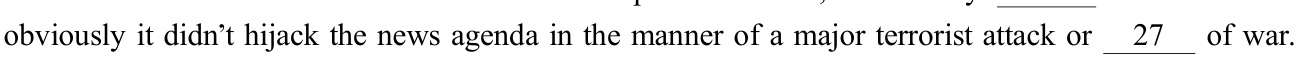
\includegraphics[width=\linewidth,height=.8\textheight,keepaspectratio]{2020-07-01.assets/char-004-line-017.png}\par

The report from the Intergovernmental Science-Policy Platform on Biodiversity and Ecosystem


\noindent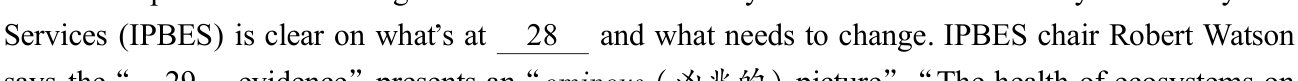
\includegraphics[width=\linewidth,height=.8\textheight,keepaspectratio]{2020-07-01.assets/char-005-line-001.png}\par

says the “ \uline{29} evidence” presents an “ominous (凶兆的) picture”. “The health of ecosystems on which we and all other species depend is \uline{30} more rapidly than ever,” Robert Watson said. “We are \uline{31} the very foundations of our economies, livelihoods, food security, health and quality of


\noindent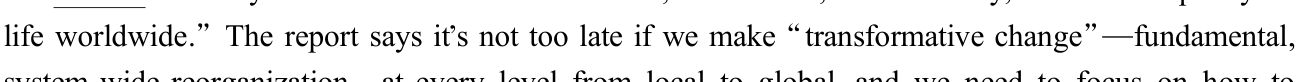
\includegraphics[width=\linewidth,height=.8\textheight,keepaspectratio]{2020-07-01.assets/char-005-line-003.png}\par

system-wide reorganization—at every level from local to global,and we need to focus on how to make that happen.


\noindent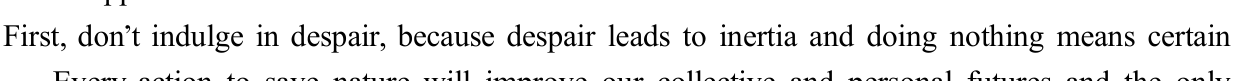
\includegraphics[width=\linewidth,height=.8\textheight,keepaspectratio]{2020-07-01.assets/char-005-line-005.png}\par

\uline{32} . Every action to save nature will improve our collective and personal futures and the only way to respond to a threat of this scale is with \uline{33} action rooted in headstrong optimism. Second, we need relentless focus, just like when paramedics (救护人员) arrive on a scene and use the concept of “triage (伤员鉴别分类)” to ensure the most \uline{34} cases get treated first. Saving the natural


\noindent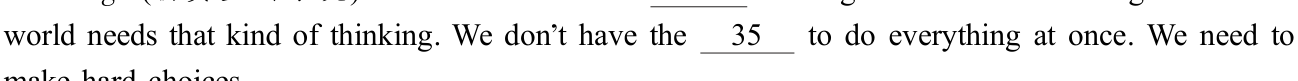
\includegraphics[width=\linewidth,height=.8\textheight,keepaspectratio]{2020-07-01.assets/char-005-line-007.png}\par

make hard choices.


\begin{itemize}[leftmargin=2em,itemsep=.2em,topsep=.4em]\item[A.] capacity
\item[B.] declaration
\item[C.] deteriorating
\item[D.] determined
\item[E.] disaster
\item[F.] eroding
\item[G.] grabbed
\item[H.] inventory
\item[I.] junction
\item[J.] monotonous
\item[K.] overwhelming
\item[L.] stagnation
\item[M.] stake
\item[N.] stifled
\item[O.] urgent
\end{itemize}

\subsection*{Section B}


Directions: In this section, you are going to read a passage with ten statements attached to it. Each statement contains information given in one of the paragraphs. Identify the paragraph from which the information is derived. You may choose a paragraph more than once. Each paragraph is marked with a letter. Answer the questions by marking the corresponding letter on Answer Sheet 2.


Children Understand Far More About Other Minds Than Long Believed


A) Until a few decades ago, scholars believed that young children know very little, if anything, about what others are thinking. Swiss psychologist Jean Piaget, who is credited with founding the


\noindent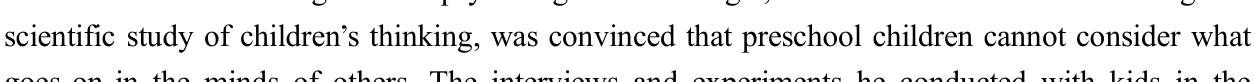
\includegraphics[width=\linewidth,height=.8\textheight,keepaspectratio]{2020-07-01.assets/char-005-line-014.png}\par

goes on in the minds of others. The interviews and experiments he conducted with kids in the middle of the 20th century suggested that they were trapped in their subjective viewpoints,


incapable of imagining what others think, feel or believe.


\noindent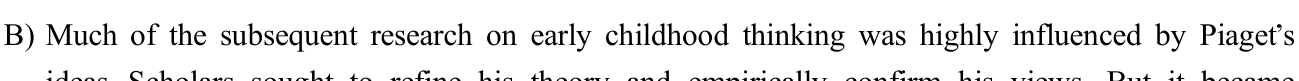
\includegraphics[width=\linewidth,height=.8\textheight,keepaspectratio]{2020-07-01.assets/char-006-line-001.png}\par

ideas. Scholars sought to refine his theory and empirically confirm his views. But it became increasingly clear that Piaget seemed to have gravely underestimated the intellectual powers of very young kids before they can make themselves understood by speech. Researchers began to devise ever more ingenious ways of figuring out what goes on in the minds of babies, and the


\noindent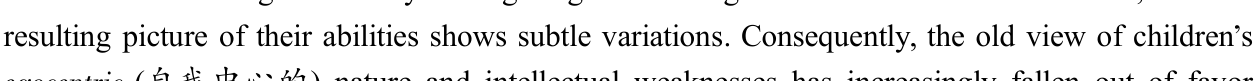
\includegraphics[width=\linewidth,height=.8\textheight,keepaspectratio]{2020-07-01.assets/char-006-line-003.png}\par

egocentric (自我中心的) nature and intellectual weaknesses has increasingly fallen out of favor and become replaced by a more generous position that sees a budding sense not only of the physical world but also of other minds, even in the “youngest young.”


\noindent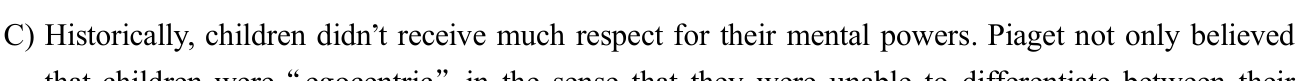
\includegraphics[width=\linewidth,height=.8\textheight,keepaspectratio]{2020-07-01.assets/char-006-line-005.png}\par

that children were “egocentric” in the sense that they were unable to differentiate between their own viewpoint and that of others; he was also convinced that their thinking was characterized by


\noindent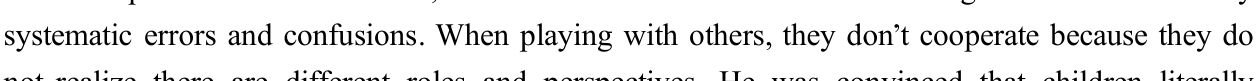
\includegraphics[width=\linewidth,height=.8\textheight,keepaspectratio]{2020-07-01.assets/char-006-line-007.png}\par

not realize there are different roles and perspectives. He was convinced that children literally cannot “get their act together”: instead of playing cooperatively and truly together, they play side by side, with little regard for others. And when speaking with others, a young child supposedly


\noindent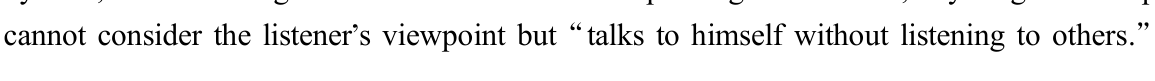
\includegraphics[width=\linewidth,height=.8\textheight,keepaspectratio]{2020-07-01.assets/char-006-line-009.png}\par

D) Piaget and his followers maintained that children go through something like a dark age of intellectual development before slowly and gradually becoming enlightened by reason and rationality as they reach school age. Alongside this enlightenment develops an ever growing understanding of other persons, including their attitudes and views of the world.


\noindent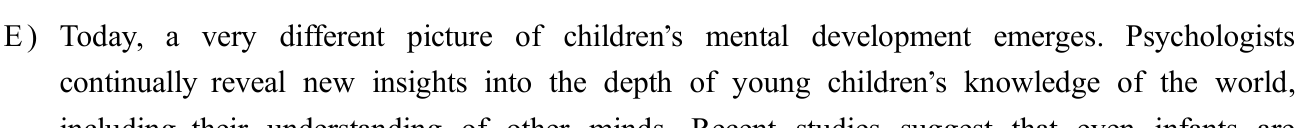
\includegraphics[width=\linewidth,height=.8\textheight,keepaspectratio]{2020-07-01.assets/char-006-line-011.png}\par

including their understanding of other minds. Recent studies suggest that even infants are


\noindent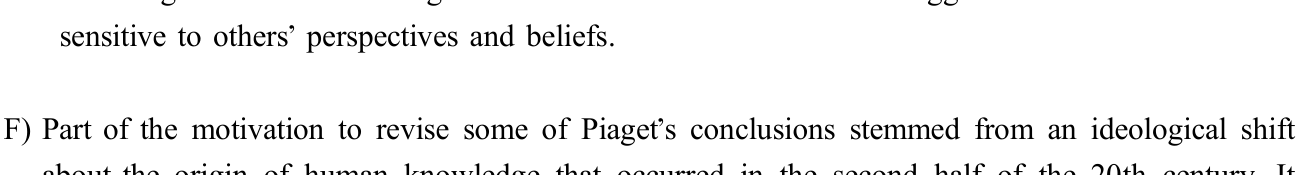
\includegraphics[width=\linewidth,height=.8\textheight,keepaspectratio]{2020-07-01.assets/char-006-line-013.png}\par

about the origin of human knowledge that occurred in the second half of the 20th century. It became increasingly unpopular to assume that a basic understanding of the world can be built entirely from experience. This was in part prompted by theorist Noam Chomsky, who argued that something as complex as the rules of grammar cannot be picked up from exposure to speech, but is supplied by an inborn “language faculty.” Others followed suit and defined further “core areas” in which knowledge allegedly cannot be pieced together from experience but must be possessed at


\noindent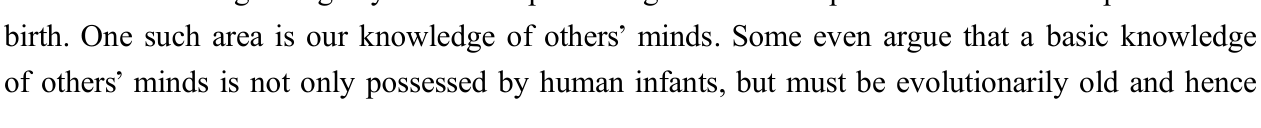
\includegraphics[width=\linewidth,height=.8\textheight,keepaspectratio]{2020-07-01.assets/char-006-line-015.png}\par

shared by our nearest living relatives, the great apes.


G) To prove that infants know more in this realm than had been acknowledged, researchers needed to come up with innovative ways of showing it. A big part of why we now recognize so much more


\noindent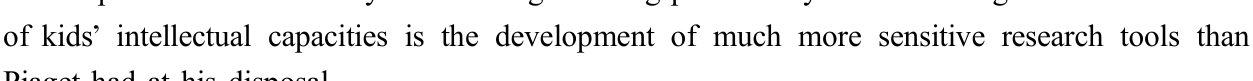
\includegraphics[width=\linewidth,height=.8\textheight,keepaspectratio]{2020-07-01.assets/char-007-line-002.png}\par

Piaget had at his disposal.


\begin{itemize}[leftmargin=2em,itemsep=.2em,topsep=.4em]\item[H.] Instead of engaging babies in dialog or having them execute complex motor tasks, the newer
\end{itemize}

\noindent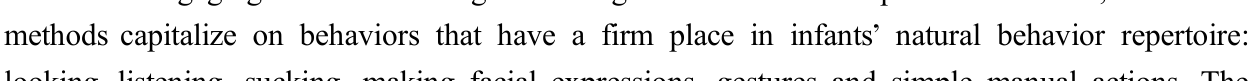
\includegraphics[width=\linewidth,height=.8\textheight,keepaspectratio]{2020-07-01.assets/char-007-line-005.png}\par

looking, listening, sucking, making facial expressions, gestures and simple manual actions. The idea of focusing on these “small behaviors” is that they give kids the chance to demonstrate their knowledge implicitly and spontaneously without having to respond to questions or instructions. For example, children might look longer at an event that they did not expect to happen, or they might show facial expressions indicating that they have sympathetic concern for others. When researchers measure these less demanding, and often involuntary, behaviors, they can detect a


\noindent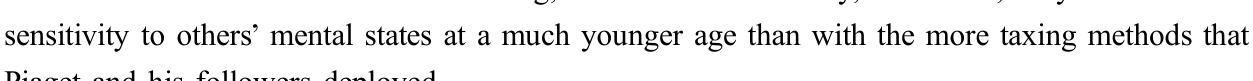
\includegraphics[width=\linewidth,height=.8\textheight,keepaspectratio]{2020-07-01.assets/char-007-line-007.png}\par

Piaget and his followers deployed.


\begin{itemize}[leftmargin=2em,itemsep=.2em,topsep=.4em]\item[I.] In the 1980s, these kinds of implicit measures became customary in developmental psychology. But
\end{itemize}

\noindent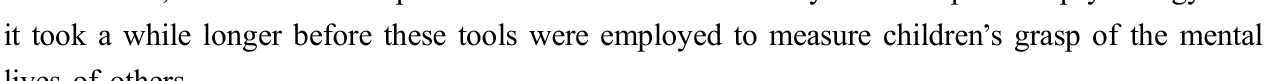
\includegraphics[width=\linewidth,height=.8\textheight,keepaspectratio]{2020-07-01.assets/char-007-line-010.png}\par

lives of others.


J) In a set of experiments, my colleagues at the University of Southern California and I found evidence that babies can even anticipate how others will feel when their expectations are disappointed. We acted out several puppet (木偶) shows in front of two-year-old children. In these puppet shows, a protagonist (Cookie Monster) left his precious belongings (cookies) on stage and later returned to fetch them. What the protagonist did not know was that an antagonist had come and messed with his possessions. The children had witnessed these acts and attentively watched the


\noindent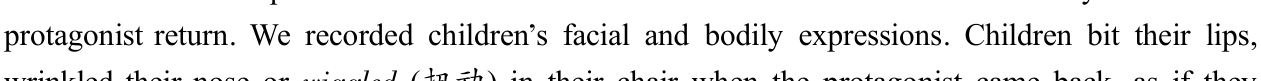
\includegraphics[width=\linewidth,height=.8\textheight,keepaspectratio]{2020-07-01.assets/char-007-line-013.png}\par

wrinkled their nose or wiggled (扭动) in their chair when the protagonist came back, as if they anticipated the bewilderment and disappointment he was about to experience. Importantly, children showed no such reactions and remained calm when the protagonist had seen the events himself and thus knew what to expect. Our study reveals that by the tender age of two, kids not only track what others believe or expect; they can even foresee how others will feel when they discover reality.


\noindent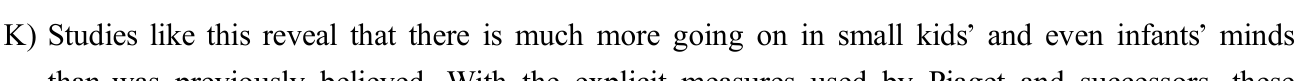
\includegraphics[width=\linewidth,height=.8\textheight,keepaspectratio]{2020-07-01.assets/char-007-line-015.png}\par

than was previously believed. With the explicit measures used by Piaget and successors, these


\noindent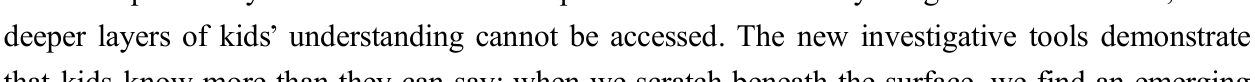
\includegraphics[width=\linewidth,height=.8\textheight,keepaspectratio]{2020-07-01.assets/char-007-line-017.png}\par

that kids know more than they can say: when we scratch beneath the surface, we find an emerging


understanding of relations and perspectives that Piaget probably did not dream of.


\noindent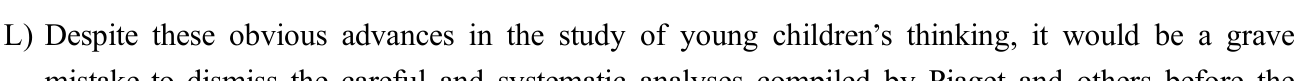
\includegraphics[width=\linewidth,height=.8\textheight,keepaspectratio]{2020-07-01.assets/char-008-line-001.png}\par

mistake to dismiss the careful and systematic analyses compiled by Piaget and others before the new tests dominated the scene because the original methods revealed essential facts about how children think that the new methods cannot uncover.


\noindent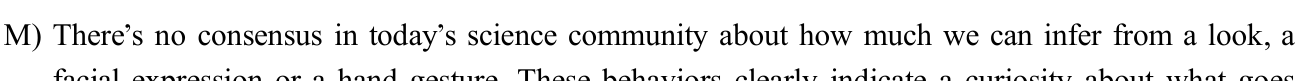
\includegraphics[width=\linewidth,height=.8\textheight,keepaspectratio]{2020-07-01.assets/char-008-line-003.png}\par

facial expression or a hand gesture. These behaviors clearly indicate a curiosity about what goes on in the mind of others, and probably a set of early intuitions coupled with a willingness to learn more. They pave the way to richer and more explicit forms of understanding of the minds of


\noindent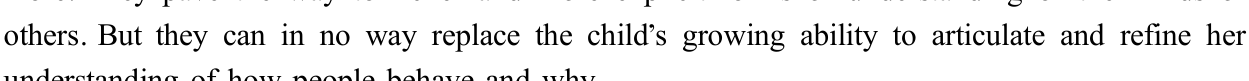
\includegraphics[width=\linewidth,height=.8\textheight,keepaspectratio]{2020-07-01.assets/char-008-line-005.png}\par

understanding of how people behave and why.


36. Piaget believed that small children could not collaborate with others while playing.


\noindent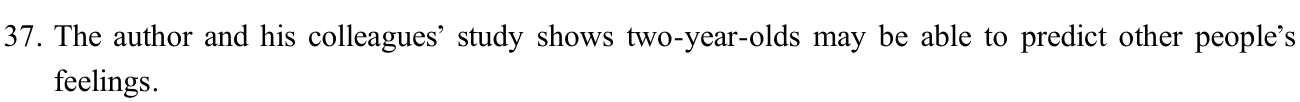
\includegraphics[width=\linewidth,height=.8\textheight,keepaspectratio]{2020-07-01.assets/char-008-line-008.png}\par

37. The author and his colleagues’ study shows two-year-olds may be able to predict other people’s feelings.


38. In the latter half of the last century, fewer and fewer people believed the basis for our understanding of the world is wholly empirical.


\noindent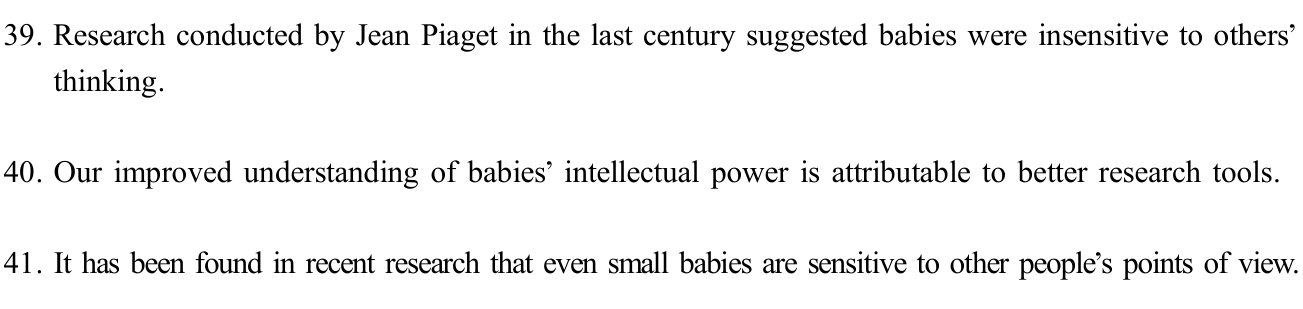
\includegraphics[width=\linewidth,height=.8\textheight,keepaspectratio]{2020-07-01.assets/char-008-line-011.png}\par

39. Research conducted by Jean Piaget in the last century suggested babies were insensitive to others’ thinking.


40. Our improved understanding of babies’ intellectual power is attributable to better research tools.


41. It has been found in recent research that even small babies are sensitive to other people’s points of view.


42. Scientists are still debating what inference can be drawn from certain physical expressions of a child.


\noindent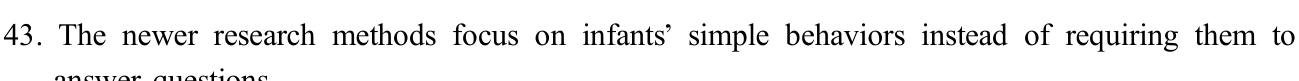
\includegraphics[width=\linewidth,height=.8\textheight,keepaspectratio]{2020-07-01.assets/char-008-line-016.png}\par

43. The newer research methods focus on infants’ simple behaviors instead of requiring them to answer questions.


\noindent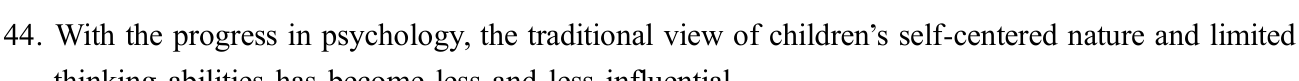
\includegraphics[width=\linewidth,height=.8\textheight,keepaspectratio]{2020-07-01.assets/char-008-line-018.png}\par

44. With the progress in psychology, the traditional view of children’s self-centered nature and limited thinking abilities has become less and less influential.


\noindent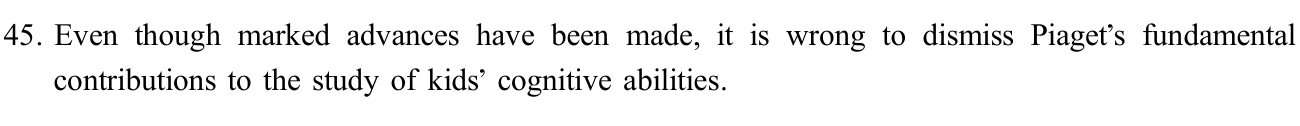
\includegraphics[width=\linewidth,height=.8\textheight,keepaspectratio]{2020-07-01.assets/char-008-line-020.png}\par

45. Even though marked advances have been made, it is wrong to dismiss Piaget’s fundamental contributions to the study of kids’ cognitive abilities.


\subsection*{Section C}


Directions: There are 2 passages in this section. Each passage is followed by some questions or unfinished statements. For each of them there are four choices marked A), B), C) and


\begin{itemize}[leftmargin=2em,itemsep=.2em,topsep=.4em]\item[D.] . You should decide on the best choice and mark the corresponding letter on Answer
\end{itemize}

Sheet 2 with a single line through the centre.


\subsection*{Passage One}


Questions 46 to 50 are based on the following passage.


People often discuss the dangers of too much stress, but lately a very different view of stress is gaining popularity: this view of stress, held by members of the positive stress movement, argues that stress might actually be beneficial. The positive stress movement is made up of people such as


\noindent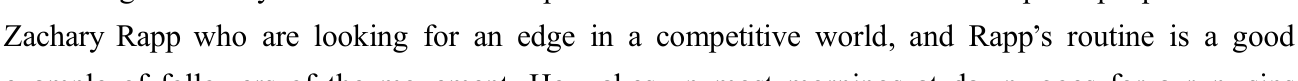
\includegraphics[width=\linewidth,height=.8\textheight,keepaspectratio]{2020-07-01.assets/char-009-line-007.png}\par

example of followers of the movement. He wakes up most mornings at dawn, goes for a run, sips black coffee while ripping through emails, and then steps into a freezing cold shower. This is a routine designed to reduce the stress of running simultaneously three different health and biotechnology companies for 18 hours a day.


\noindent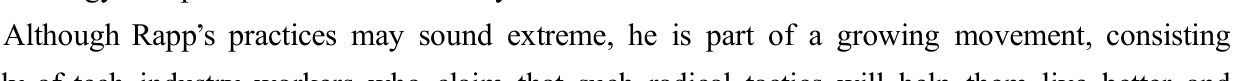
\includegraphics[width=\linewidth,height=.8\textheight,keepaspectratio]{2020-07-01.assets/char-009-line-009.png}\par

largely of tech industry workers who claim that such radical tactics will help them live better and longer. Inspired by influential figures in different fields, including entertainers, athletes, entrepreneurs and scientists, positive stress practitioners seek out some combination of extreme temperatures, restrictive diets, punishing exercise routines and general discomfort.


Rapp argues that positive stress keeps him balanced. In addition to running and freezing showers, Rapp uses ice baths, hot yoga, and unconventional eating practices such as eliminating dairy, sugar, alcohol and various other foods high in carbohydrates. He believes that these practices, which put stress on his body, actually make him feel less stress from work. However, Rapp does not credit anyone in particular for his choices: he said he started using these methods in college, where he got into the habit of taking ice baths to recover from sports. He got back into it while trying to get his three companies off the ground.


Rapp works long hours and sleeps only five to seven hours a night but he said he only gets sick once a year. For him, the difference between day-to-day stress, like the kind we feel when moving apartments, and positive stress is that the latter involves pushing the body to extremes and forcing it to build up a tolerance.


One thought leader in the positive stress world is Dutch extreme athlete Wim Hof, who earned


\noindent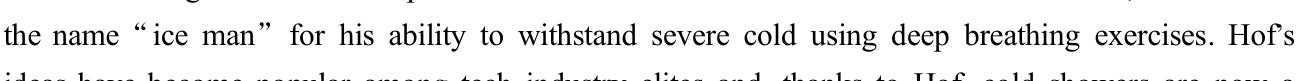
\includegraphics[width=\linewidth,height=.8\textheight,keepaspectratio]{2020-07-01.assets/char-009-line-014.png}\par

ideas have become popular among tech industry elites and, thanks to Hof, cold showers are now a trend; indeed, some even call it a form of therapy.


But it is important to note that not everyone agrees with these practitioners; indeed, some medical professionals argue that positive stress is not for everyone, and that it might even be dangerous for people who are unhealthy or older.


46. What do we learn about followers of the positive stress movement?


\begin{itemize}[leftmargin=2em,itemsep=.2em,topsep=.4em]\item[A.] They are usually quite sensitive to different types of stress.
\item[B.] They hold a different view on stress from the popular one.
\item[C.] They derive much pleasure from living a very hectic life.
\item[D.] They gain a competitive edge by enjoying good health.
\end{itemize}

47. What do followers of the positive stress movement usually do to put their ideas into practice?


\begin{itemize}[leftmargin=2em,itemsep=.2em,topsep=.4em]\item[A.] They keep changing their living habits.
\item[B.] They network with influential figures.
\item[C.] They seek jobs in tech industries.
\item[D.] They apply extreme tactics.
\end{itemize}

48. What does Zachary Rapp say about his unconventional practices?


\begin{itemize}[leftmargin=2em,itemsep=.2em,topsep=.4em]\item[A.] They help him combat stress from work.
\item[B.] They enable him to cut down living expenses.
\item[C.] They enable him to recover from injuries and illnesses.
\item[D.] They help him get three companies enlisted all at once.
\end{itemize}

49. What can be inferred from the passage about day-to-day stress?


\begin{itemize}[leftmargin=2em,itemsep=.2em,topsep=.4em]\item[A.] It is harmful to one’s physical and mental health.
\item[B.] It does not differ in essence from positive stress.
\item[C.] It is something everybody has to live with.
\item[D.] It does not help build up one’s tolerance.
\end{itemize}

50. What do some medical professionals think of positive stress?


\begin{itemize}[leftmargin=2em,itemsep=.2em,topsep=.4em]\item[A.] Its true effect remains to be verified.
\item[B.] Its side effect should not be ignored.
\item[C.] Its effect varies considerably from person to person.
\item[D.] Its practitioners should not take it as a form of therapy.
\end{itemize}

\subsection*{Passage Two}


Questions 51 to 55 are based on the following passage.


Is hunting good or bad for the environment? Like so many hot button issues, the answer to this question depends upon who you ask. On the one hand, some say, nothing could be more natural than


hunting, and indeed just about every animal species—including humans—has been either predator or prey at some point in its evolution. And, ironic as it sounds, since humans have wiped out many animal predators, some see hunting as a natural way to reduce the herds of prey animals that now


\noindent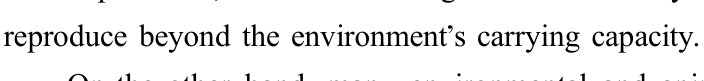
\includegraphics[width=\linewidth,height=.8\textheight,keepaspectratio]{2020-07-01.assets/char-011-line-001.png}\par

On the other hand, many environmental and animal advocates see hunting as savage, arguing that it is morally wrong to kill animals, regardless of practical considerations. According to Glenn


\noindent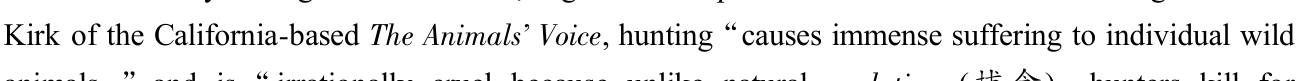
\includegraphics[width=\linewidth,height=.8\textheight,keepaspectratio]{2020-07-01.assets/char-011-line-003.png}\par

animals...” and is “ irrationally cruel because unlike natural predation (捕食), hunters kill for


\noindent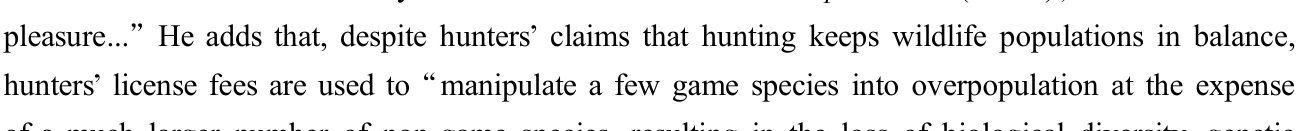
\includegraphics[width=\linewidth,height=.8\textheight,keepaspectratio]{2020-07-01.assets/char-011-line-005.png}\par

of a much larger number of non-game species, resulting in the loss of biological diversity, genetic integrity and ecological balance.”


Beyond moral issues, others contend that hunting is not practical. According to the Humane Society of the United States, the vast majority of hunted species—such as waterfowl, rabbits, upland birds and mourning doves—“provide minimal nutrition and do not require population control.”


\noindent
\includegraphics[width=\linewidth,height=.8\textheight,keepaspectratio]{2020-07-01.assets/char-011-line-008.png}\par

be morally justifiable while others may not be. Hunting “designed to secure the aggregate welfare of the target species, the integrity of its ecosystem, or both ”—what Varner terms “ therapeutic hunting”—is defensible, while subsistence and sport hunting—both of which only benefit human beings—is not.


\noindent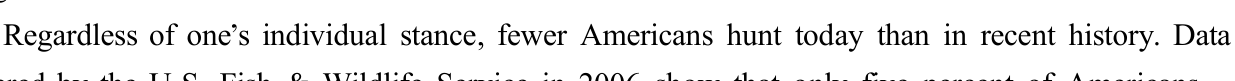
\includegraphics[width=\linewidth,height=.8\textheight,keepaspectratio]{2020-07-01.assets/char-011-line-010.png}\par

gathered by the U.S. Fish \& Wildlife Service in 2006 show that only five percent of Americans— some 12.5 million individuals—consider themselves hunters today, down from nine percent in 2001 and 15 percent in 1996.


Public support for hunting, however, is on the rise. A 2007 survey by Responsive Management Inc. found that eighty percent of respondents agreed that “hunting has a legitimate place in modern society,” and the percentage of Americans indicating disapproval of hunting declined from 22 percent in 1995 to 16 percent in 2007.


Perhaps matching the trend among the public, green leaders are increasingly advocating cooperation between hunters and environmental groups: After all, both deplore urban sprawl and habitat destruction.


51. What does the author say sounds ironic?


\begin{itemize}[leftmargin=2em,itemsep=.2em,topsep=.4em]\item[A.] Some predators may often turn out to be prey of other predators.
\item[B.] Hunting may also be a solution to the problem caused by hunting.
\item[C.] The species of prey animals continue to vary despite humans’ hunting.
\item[D.] The number of prey animals keeps rising despite environmental change.
\end{itemize}

52. What does Glenn Kirk think of charging hunters license fees?


\begin{itemize}[leftmargin=2em,itemsep=.2em,topsep=.4em]\item[A.] It keeps game population under control.
\item[B.] It turns hunting into a sport of the rich.
\item[C.] It leads to ecological imbalance.
\item[D.] It helps stop killing for pleasure.
\end{itemize}

53. What is the argument of the Humane Society of the United States against hunting?


\begin{itemize}[leftmargin=2em,itemsep=.2em,topsep=.4em]\item[A.] Overpopulation is not an issue for most hunted animals.
\item[B.] Hunting deprives animal populations of their food sources.
\item[C.] Many birds and small animals are being irrationally killed.
\item[D.] Hunting is universally acknowledged as a savage behavior.
\end{itemize}

54. When is hunting morally justifiable according to Gary E. Varner?


\begin{itemize}[leftmargin=2em,itemsep=.2em,topsep=.4em]\item[A.] When it benefits animals and their ecosystem.
\item[B.] When it serves both human and animal interests.
\item[C.] When it is indispensable to humans’ subsistence.
\item[D.] When it stabilizes the population of animal species.
\end{itemize}

55. What concept are green leaders trying to promote?


\begin{itemize}[leftmargin=2em,itemsep=.2em,topsep=.4em]\item[A.] Effective protection of animal habitats.
\item[B.] Strict control over urban development.
\item[C.] Coordinated efforts of hunters and environmentalists.
\item[D.] A compromise between development and animal protection.
\end{itemize}

\subsection*{Part IV Translation (30 minutes)}


Directions: For this part, you are allowed 30 minutes to translate a passage from Chinese into


English. You should write your answer on Answer Sheet 2.


《\CJKunderline{三国演义}》(The Romance of the Three Kingdoms)是中国一部著名的历史小说,写于十四世纪。这部文学作品以三国时期的历史为背景,描写了从公元二世纪下半叶到公元三世纪下半叶的魏、蜀、吴三国之间的战争。小说中刻画了近千个人物和无数的历史事件。这些人物和事件虽然大都基于真实的历史,但都不同程度地被浪漫化和戏剧化了。《三国演义》是一部公认的文学杰作。自面世以来,这部小说不断吸引着一代又一代的读者,并且对中国文化产生了广泛而持久的影响。


\begin{center}
\includegraphics[width=.85\linewidth,height=.55\textheight,keepaspectratio]{2020-07-01.assets/figure-013-000.png}\end{center}

I I I I I I I I I I I I I I I I

\end{document}